%%
%% This is file `sigconf.tex',
%% generated with the docstrip utility.
%%
%% The original source files were:
%%
%% samples.dtx  (with options: `all,proceedings,sigconf')
%% 
%% IMPORTANT NOTICE:
%% 
%% For the copyright see the source file.
%% 
%% Any modified versions of this file must be renamed
%% with new filenames distinct from sigconf.tex.
%% 
%% For distribution of the original source see the terms
%% for copying and modification in the file samples.dtx.
%% 
%% This generated file may be distributed as long as the
%% original source files, as listed above, are part of the
%% same distribution. (The sources need not necessarily be
%% in the same archive or directory.)
%%
%%
%% Commands for TeXCount
%TC:macro \cite [option:text,text]
%TC:macro \citep [option:text,text]
%TC:macro \citet [option:text,text]
%TC:envir table 0 1
%TC:envir table* 0 1
%TC:envir tabular [ignore] word
%TC:envir displaymath 0 word
%TC:envir math 0 word
%TC:envir comment 0 0
%%
%% The first command in your LaTeX source must be the \documentclass
%% command.
%%
%% For submission and review of your manuscript please change the
%% command to \documentclass[manuscript, screen, review]{acmart}.
%%
%% When submitting camera ready or to TAPS, please change the command
%% to \documentclass[sigconf]{acmart} or whichever template is required
%% for your publication.
%%
%%
\documentclass[sigconf]{acmart}
\settopmatter{printacmref=false}
\renewcommand\footnotetextcopyrightpermission[1]{}
%%
%% \BibTeX command to typeset BibTeX logo in the docs
\AtBeginDocument{%
  \providecommand\BibTeX{{%
    Bib\TeX}}}

%% Rights management information.  This information is sent to you
%% when you complete the rights form.  These commands have SAMPLE
%% values in them; it is your responsibility as an author to replace
%% the commands and values with those provided to you when you
%% complete the rights form.
%% \setcopyright{Chris Humphreys}
%% \copyrightyear{2026}
%% \acmYear{2026}
%% \acmDOI{XXXXXXX.XXXXXXX}
%% These commands are for a PROCEEDINGS abstract or paper.
\acmConference[2026 GATech CyberSecurity Masters Practicum]
              {2026 GATech CyberSecurity Masters Practicum}{2026}{Atlanta, GA}
%%
%%  Uncomment \acmBooktitle if the title of the proceedings is different
%%  from ``Proceedings of ...''!
%%
\acmBooktitle{2026 GATech CyberSecurity Masters Practicum}
\acmISBN{}


%%
%% Submission ID.
%% Use this when submitting an article to a sponsored event. You'll
%% receive a unique submission ID from the organizers
%% of the event, and this ID should be used as the parameter to this command.
%%\acmSubmissionID{123-A56-BU3}

%%
%% For managing citations, it is recommended to use bibliography
%% files in BibTeX format.
%%
%% You can then either use BibTeX with the ACM-Reference-Format style,
%% or BibLaTeX with the acmnumeric or acmauthoryear sytles, that include
%% support for advanced citation of software artefact from the
%% biblatex-software package, also separately available on CTAN.
%%
%% Look at the sample-*-biblatex.tex files for templates showcasing
%% the biblatex styles.
%%
%%
%% The majority of ACM publications use numbered citations and
%% references.  The command \citestyle{authoryear} switches to the
%% "author year" style.
%%
%% If you are preparing content for an event
%% sponsored by ACM SIGGRAPH, you must use the "author year" style of
%% citations and references.
%% Uncommenting
%% the next command will enable that style.
%%\citestyle{acmauthoryear}


%%
%% end of the preamble, start of the body of the document source.
\begin{document}

%%
%% The "title" command has an optional parameter,
%% allowing the author to define a "short title" to be used in page headers.
\title{Efficient Identification of Malicious Advertisements in Search Results}

%%
%% The "author" command and its associated commands are used to define
%% the authors and their affiliations.
%% Of note is the shared affiliation of the first two authors, and the
%% "authornote" and "authornotemark" commands
%% used to denote shared contribution to the research.
%% \author{Ben Trovato}
%% \authornote{Both authors contributed equally to this research.}
%% \email{trovato@corporation.com}
%% \orcid{1234-5678-9012}
%% \author{G.K.M. Tobin}
%% \correspondingauthor
%% \authornotemark[1]
%% \email{webmaster@marysville-ohio.com}
%% \affiliation{%
%%   \institution{Institute for Clarity in Documentation}
%%   \city{Dublin}
%%   \state{Ohio}
%%   \country{USA}
%% }

\author{Chris Humphreys}
\affiliation{%
  \institution{Georgia Institute of Technology}
  \city{Atlanta}
  \country{United States}}
\email{chumphreys8@gatech.edu}

%%
%% By default, the full list of authors will be used in the page
%% headers. Often, this list is too long, and will overlap
%% other information printed in the page headers. This command allows
%% the author to define a more concise list
%% of authors' names for this purpose.
%% \renewcommand{\shortauthors}{Trovato et al.}

%%
%% The abstract is a short summary of the work to be presented in the
%% article.
\begin{abstract}
  The problem of malicious advertisements in search engine result pages (SERP)
  is not a new development, but the recent rise in popularity of the ClickFix
  technique and its associated use of malvertising
  \cite{abrams_2026_cluade_clickfix} demonstrate that the technique is still
  being used and seeing success.
  Unfortunately, other than a few exceptions \cite{kumari_2024_ml_classification}
  \cite{huang_2020_bayesian_game}\cite{blancaflor_2024_ai_chat}, there has been
  very little academic research into the prevalence of malicious advertising
  over the last 10 year period in general, and even less in regards to search
  engine result page (SERP) specific malvertising. This research presents a
  tested process for capturing and analyzing advertisements and testing them for
  signs of maliciousness. This is achieved through the use of an automated,
  multi-threaded SERP collection system which uses 4 distinct oracles for final
  analysis.
  Critically, it does this in a very fast and efficient
  manner with a focus on asynchronously pulling the website data that is needed
  for analysis, but nothing more.
  I was able to collect and analyze over 14,000 queries in a timeframe of less
  than 6 hours, but I did not identify any malicious advertisements.
  This null result suggests that current malvertising cloaking techniques
  are robust, and also that more research is warranted.
  The tools developed in this research will give future analysts
  a strong head start in their efforts to further their study of this topic.
\end{abstract}

%%
%% The code below is generated by the tool at http://dl.acm.org/ccs.cfm.
%% Please copy and paste the code instead of the example below.
%%
%% \begin{CCSXML}
%% <ccs2012>
%%  <concept>
%%   <concept_id>00000000.0000000.0000000</concept_id>
%%   <concept_desc>Do Not Use This Code, Generate the Correct Terms for Your Paper</concept_desc>
%%   <concept_significance>500</concept_significance>
%%  </concept>
%%  <concept>
%%   <concept_id>00000000.00000000.00000000</concept_id>
%%   <concept_desc>Do Not Use This Code, Generate the Correct Terms for Your Paper</concept_desc>
%%   <concept_significance>300</concept_significance>
%%  </concept>
%%  <concept>
%%   <concept_id>00000000.00000000.00000000</concept_id>
%%   <concept_desc>Do Not Use This Code, Generate the Correct Terms for Your Paper</concept_desc>
%%   <concept_significance>100</concept_significance>
%%  </concept>
%%  <concept>
%%   <concept_id>00000000.00000000.00000000</concept_id>
%%   <concept_desc>Do Not Use This Code, Generate the Correct Terms for Your Paper</concept_desc>
%%   <concept_significance>100</concept_significance>
%%  </concept>
%% </ccs2012>
%% \end{CCSXML}

%% \ccsdesc[500]{Do Not Use This Code~Generate the Correct Terms for Your Paper}
%% \ccsdesc[300]{Do Not Use This Code~Generate the Correct Terms for Your Paper}
%% \ccsdesc{Do Not Use This Code~Generate the Correct Terms for Your Paper}
%% \ccsdesc[100]{Do Not Use This Code~Generate the Correct Terms for Your Paper}

%%
%% Keywords. The author(s) should pick words that accurately describe
%% the work being presented. Separate the keywords with commas.
%% \keywords{Do, Not, Use, This, Code, Put, the, Correct, Terms, for,
%%   Your, Paper}
%% A "teaser" image appears between the author and affiliation
%% information and the body of the document, and typically spans the
%% page.
%% \begin{teaserfigure}
%%  \includegraphics[width=\textwidth]{sampleteaser}
%%   \caption{Seattle Mariners at Spring Training, 2010.}
%%   \Description{Enjoying the baseball game from the third-base
%%   seats. Ichiro Suzuki preparing to bat.}
%%   \label{fig:teaser}
%% \end{teaserfigure}

%% \received{20 February 2007}
%% \received[revised]{12 March 2009}
%% \received[accepted]{5 June 2009}

%%
%% This command processes the author and affiliation and title
%% information and builds the first part of the formatted document.
\maketitle

\section{Introduction}
Malicious advertisements in general are not a new problem and have
been reported on as early as 2009 when hackers
broke into the New York Times banner feed and displayed fake ads that implied
potential victims systems were infected. \cite{picchi_2009_malvertising}
Any tool that allows users the ability to create their own ads has the potential
for abuse, and the auction style system with minimal human oversight used by
organizations like Google are no exception to this.
In fact, adversaries have been observed creating malicious advertisiements on
Google search results that are purportedly for Chrome, a Google owned web
browser, but in actuality led to the installation of malware.
\cite{peters_2016_gooogle_adwords}

While the technique is around 20 years old at this point, adversaries continue
to see success using it.
As recently as October of 2026, fake advertsiements for Claude installers were
being used as pretext to get victims to visit sites that spread malware via
ClickFix, a social engineering technique in which the victims are tricked into
copying, pasting, and executing malicious commands on their own systems.
\cite{abrams_2026_cluade_clickfix}

The benefit of using search engine result page advertisements for malicious
puproses over other forms of advertising is that the search provider name lends
legitimacy to the advertisments visible on the results page, whether warranted
or not.
In addition to this, the fake advertisement can be for whatever product the
adversary wants to show and often, as above, common trusted applications are
used for this purpose.
Google and other providers do attempt to minimize the number of malicious ads,
but the fact that content on the web can be modified at will makes this next to
impossible.
As an example, a malicious actor could create an ad that points to a completely
benign webpage, and once the approval process is complete, the redirect chain
could be modified, DNS could be updated, or the content of the site could be
updated to begin serving malicious content.

Over the last 10 years or so the amount of academic research on this topic has
waned.
Up until 2017 there were a number of researchers looking into and publishing
research on malicious advertisements, but that output has slowed dramatically.
Another goal of this work is to update and modernize the tools and techniques
that have been neglected.

This paper will detail a the workings and use of a Python application created to
identify malicious advertisements presented on Google Search Engine Results
Pages (SERP).
In Section~\ref{sec:background} we review how these malicious ads work and
Section~\ref{sec:related_work} will examine the existing literature on this
topic. Section~\ref{sec:methodology} describes the architecture of the
application and its tooling in detail.
My findings are presented in Section~\ref{sec:results}, and Future Work and
Conlcusions can be found in Sections~\ref{sec:future_work}
and \ref{sec:conclusion}.

\section{Background}
\label{sec:background}
A threat actor's ultimate goal is access to the system of an unsuspecting
victim.
Abusing search engine result page advertising networks for intial access
vectors that can both filter the potential victim pool to
users who are most likely to match the attackers ideal target profile, and lend
legitimacy by being presented to the victim in the context of an otherwise
trusted web site is an effective way that threat actors gain an inital foothold.

Malicious actors are able to  select the target profile of who the ads are being
presented to, thereby narrowing the potential victim pool before the attack even
begins.
Items such as interests and habits, what a person is actively searching for and
more can be selected by the adversary\cite{google_2026_ad_docs}, and the fact
that these ads are seen on an otherwise trusted site like Google gives these
malicious ads a false sense safety.
These factors have been exploited in attacks that use malicious
advertising as a part of the attack chain such as recent ClickFix campaigns~\cite{huntress_2026_evolving_clickfix}. 

Cloaking is the term most commonly used to describe adversarial attempts to
evade detection efforts.
Invernizzi et al.~\cite{invernizzi_2016_cloak} note that cloaking relies on the
fact that ``not every client observes the same content''.
This fact is exploited to display benign content to researchers and law
enforcement, but malicious websites to potential victims.

Between the first query submission and the initial access of a victims's system
a number of steps take place as illustrated in figure~\ref{fig:ad_workflow}.
Each of these steps presents a unique challenges to researchers who working to
study the issue of malvertising.

\begin{figure}[htbp]
  \centering
  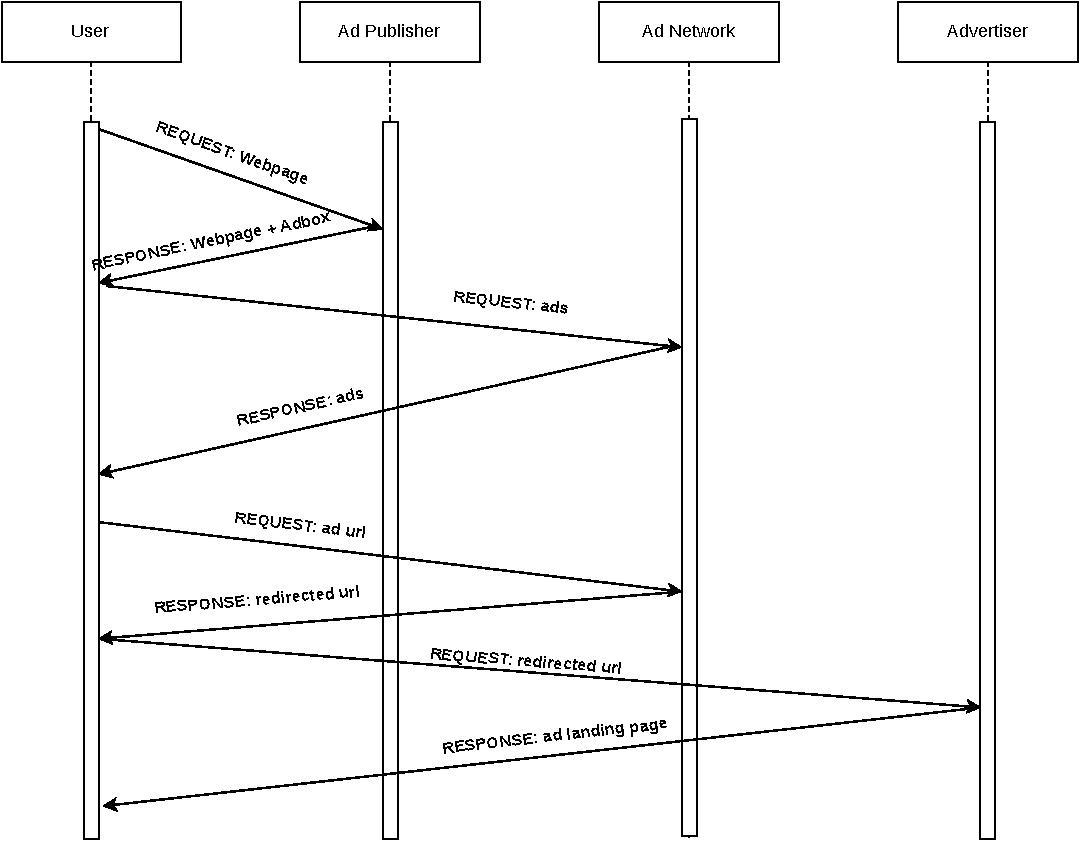
\includegraphics[width=\columnwidth]{advertising_workflow.pdf}
  \caption{Overview of the malvertising delivery workflow, adapted from Sakib
    and Huang~\cite{sakib_2015_automated_collection}.}
  \label{fig:ad_workflow}
\end{figure}

The first hurdle to collecting malicious advertisements is that of collecting
any advertisements, malicious or not, to analyze.
While in normal browsing it can seem as if every action taken results in a huge
number of advertisements being presented.
Study of the issue, and attempts to purposely generate advertisements on SERP's,
demonstrate that this is not as
straightforward as it may initially be thought.
Many search engine queries in fact present no advertisements at all.
The line in figure~\ref{fig:ad_workflow} labeled ``RESPONSE: ads'' is an
empty response that contains no advertisements at all more often than not. 

These initial ad URL's are not actually direct links to the products and
services being advertised as is often assumed.
Rather, these URLS first request the actual ad URL from Google (or whatever ad
provider is supplying them).
Behind the scenes the ad network provider is notified that an ad URL has been
clicked, which they note for billing and tracking puproses, and then a vendor
provded URL is returned.
This is illustrated in the four lowermost arrows in
figure~\ref{fig:ad_workflow}.

One important consideration in this work is the efficiency of the total process.
The vast majority of advertisements are legitimate so even putting aside
cloaking and other known roadblocks, finding a malcious ad in a sea of
legitimate ones is akin to searching for a needle in a haystack.
One of the goals of this research is to find a way to quicky analyze the ads, or
the haystack.
Essentially, the more hay can be analyzed, the better chance of idenitfying the
needle, or the haystack.

\section{Related Work}
\label{sec:related_work}
Just a couple paragraphs here with links to the articles I reviewed.

\section{Methodology}
\label{sec:methodology}
This work is largely based around 4 modules that create a pipeline
of analysis steps that start with an inital query to a search engine, and result
in an output that counts the number of advertisements with signs of
malciousness.

The first of the four modules utilized in this workflow are the Executor, which
is an orchestrator and provides high level methods and functionality.
The Executor is the interface with which the user directly interacts.
The Collector, as the name suggests, collects the intial ad URL's presented to
the user on the SERP.
Once these URL's have been collected, it is the Detector module that follows any
redirects and pulls the final landing page.
The Classifier then runs the collected web content against the four oracles, and
returns final analysis to the Executor who then provides the information to the
user.

\paragraph{Cost and Billing Considerations}
Implementation of resources that have monetary costs (SERP Provider API and
Residential Proxy Access) has been done deliberately with a goal of minimizing
costs as much as possible.
Some of the steps taken to assist in this are as follows, each ad URL is
resolved only once, anything that can be done offline or with free tools is done
in that manner, and the number of resources pulled with each site is minimized
as much as possible.  This last item was achieved through not pulling items
like images, video, and other assets when the ad URLs are resolved.
These results can be recreated by subscribing to the lowest usage tiers of
Oxylabs SERP API and Residential Proxy offerings.
A single month subscription to both of these services is currently less that one
hundred US Dollars.

\subsection{System Design}

This system design was intentionally created to be able to bypass as
many cloaking techniques as possible, while still running quicly and at a low
cost, both monetarily and in terms of other resources.

\begin{figure}[htbp]
  \centering
  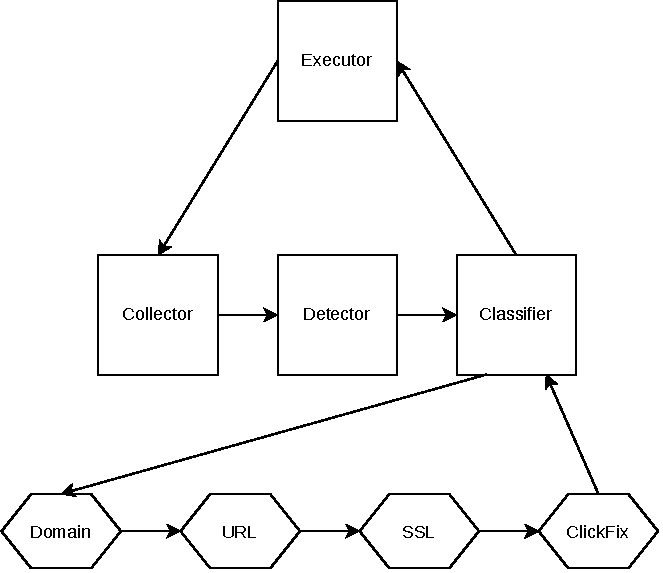
\includegraphics[width=\columnwidth]{workflow.pdf}
  \caption{Overall workflow and module interaction.}
  \label{fig:final_workflow}
\end{figure}

Figure~\ref{fig:final_workflow} shows how these pieces fit together and the
direction in which the data moves as it is processed and resolved.
Each of these modules and the four oracles are examined in detail next.

\subsubsection{Collector Object}
Describe object goal -> collect Ad URLS
- Good spot to review how ad urls work again

How and why I dropped metadata and images to get faster response.

Why I had to use a SERP and what that is.

Talk about User-Agents and cloaking avoidance

Discuss how multi-threaded aspect works

Oxylabs API integration and costs
- JSON response
- Could be used with other API providers

what data is returned and in what form
- Ad Urls in a list

\subsubsection{Detector Object}
Describe ojbect goal -> resolve URLs to final landing pages

How and why I dropped metadata and images to get faster response.
- also lowered total costs

Why I had to use residential proxies and what that is.

Discuss playwright and playwright stealth and advantages over requests library.
- Talk about what playwright can drop
- Discuss JS redirects and how playwright can resolve.

Asynchronous architecture and how that allows for multiple concurrent requests.

Residential proxy API and costs
- How responses look
- Integrations with other API Providers

What data is returned in what form
- dict of ad info (describe fields)

Advertising Diagram with Modules show

\begin{figure}[htbp]
  \centering
  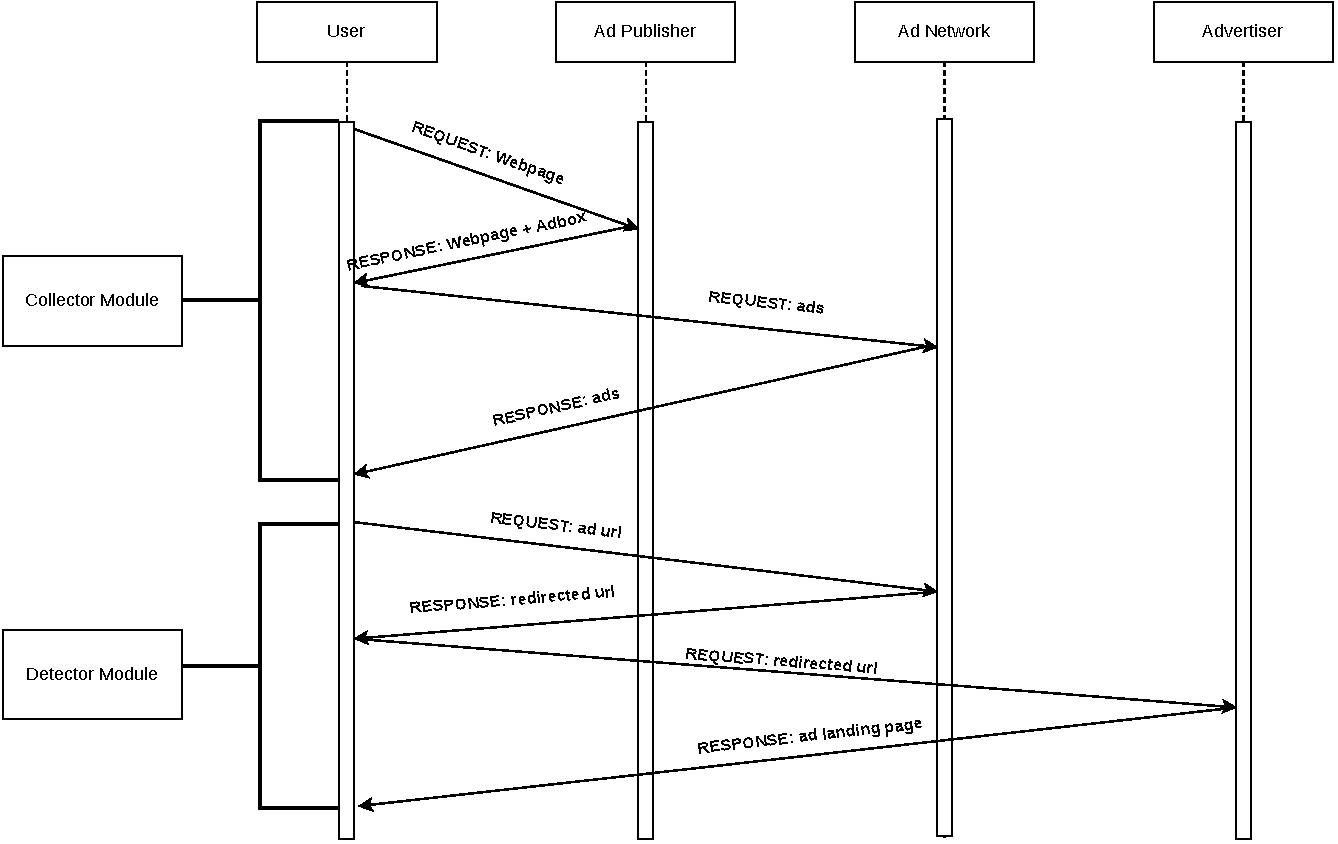
\includegraphics[width=\columnwidth]{advertising_workflow_modules.pdf}
  \caption{Overview of the malvertising delivery workflow including collector
    and detector modules, adapted from Sakib and
    Huang~\cite{sakib_2015_automated_collection}.}
  \label{fig:ad_workflow_modules}
\end{figure}

\subsubsection{Classifier Object}
Describe Object goal -> assess using classifiers

Discuss what data is returned and in what form

\subsubsection{Oracles}
\begin{itemize}
\item Domain BlockList Oracle
  What it is (detials like how many domains included)
  Where I got it from
  how often it is updated
  How analysis is done
  FP's -> what they look like and how they show the oracle works
\item URLHaus Oracle
  What it is (details like how many URLs included)
  Where I got it from
  - Mention that you need an accoutn at URLHaus
  how often it is updated
  How analysis is done
\item SSL Oracle
  What it is
  Some sort of citation to use to justify that SSL certs are new in malvertising
  How analysis is done
  - Maybe worth mentioning UNIX timestamps from epoch
  FP's what they look like and how they show the oracle works
\item ClickFix Oracle
  What it is and goals
  How JS puts stuff into the clipboard
  How analysis is done
  FP's what they look like and how they show the oracle works
\end{itemize}

\subsection{Executor}
Brief overview of additional functionality provided.

Disucssion of CLI options

\subsection{Queries}
Review the three query sources and justify each one.
- If used in previous work, mention the older results
Talk about expectations of each query set.

\section{Results}
\label{sec:results}
Discuss how my expirement ran
- date
- time taken
- number of queries executed
- Interpreter and methods used

Review what the output looks like (what form)
include screenshot if it will be helpful.

\subsection{Findings}
No ads found :(
- Cloacking
- Short time frames malicious ads run
- Query coverage

summarize what was done (number of queires executes)

Compare number of ads found across query sources
- good spot for a bar graph to illustrate.

Compare number of failed responses across the three query sets
- another good spot for a graph

\subsection{Comparisons to previous work}
May not use this, we will see.  not sure if there is enough direct comparisons
to warrant an entire subsection.

\section{Future Work}
\label{sec:future_work}
Useage with other search engines

Useage with otehr API providers

New or different oracles, easy to add or remove, each is a method.
- If cost and efficiency less important, could be useful to try more
analytically expensive comparisons.

Non-Search engine advertising analysis

Better cloaking avoidance

round the clock querying

\section{Conclusion}
\label{sec:conclusion}
Summarize everything together.

%%
%% The next two lines define the bibliography style to be used, and
%% the bibliography file.
\bibliographystyle{ACM-Reference-Format}
\bibliography{references}


%%
%% If your work has an appendix, this is the place to put it.
%% \appendix

%% \section{Research Methods}

%% \subsection{Part One}

%% Lorem ipsum dolor sit amet, consectetur adipiscing elit. Morbi
%% malesuada, quam in pulvinar varius, metus nunc fermentum urna, id
%% sollicitudin purus odio sit amet enim. Aliquam ullamcorper eu ipsum
%% vel mollis. Curabitur quis dictum nisl. Phasellus vel semper risus, et
%% lacinia dolor. Integer ultricies commodo sem nec semper.

%% \subsection{Part Two}

%% Etiam commodo feugiat nisl pulvinar pellentesque. Etiam auctor sodales
%% ligula, non varius nibh pulvinar semper. Suspendisse nec lectus non
%% ipsum convallis congue hendrerit vitae sapien. Donec at laoreet
%% eros. Vivamus non purus placerat, scelerisque diam eu, cursus
%% ante. Etiam aliquam tortor auctor efficitur mattis.

%% \section{Online Resources}

%% Nam id fermentum dui. Suspendisse sagittis tortor a nulla mollis, in
%% pulvinar ex pretium. Sed interdum orci quis metus euismod, et sagittis
%% enim maximus. Vestibulum gravida massa ut felis suscipit
%% congue. Quisque mattis elit a risus ultrices commodo venenatis eget
%% dui. Etiam sagittis eleifend elementum.

%% Nam interdum magna at lectus dignissim, ac dignissim lorem
%% rhoncus. Maecenas eu arcu ac neque placerat aliquam. Nunc pulvinar
%% massa et mattis lacinia.

\end{document}
\endinput

%% End of file `sigconf.tex'.
